\documentclass[11pt]{article}
\usepackage{fontspec}
\setmainfont{Arial}
\setsansfont{Arial}
\setmonofont{Arial}
\usepackage{unicode-math}
\setmathfont{TeX Gyre Termes Math}
\usepackage[margin=1in]{geometry}
\usepackage{amsmath}
\usepackage{graphicx}
\usepackage{booktabs}
\usepackage{multirow}
\usepackage{siunitx}
\usepackage{caption}
\usepackage{subcaption}
\usepackage{tikz}
\usetikzlibrary{arrows.meta,positioning,calc,fit,decorations.pathreplacing}
\usepackage[numbers,round]{natbib}
\usepackage[svgnames]{xcolor}
\usepackage{authblk}
\usepackage{microtype}
\usepackage{xurl}
\usepackage[hidelinks]{hyperref}

\captionsetup{font=small,labelfont=bf,skip=6pt}
\setlength{\parskip}{0.3em plus 0.1em minus 0.1em}
\setlength{\parindent}{0pt}

\newcommand{\panfig}[1]{\resizebox{\textwidth}{!}{\input{#1}}}
\newcommand{\panhalffig}[1]{\resizebox{0.98\linewidth}{!}{\input{#1}}}

\usepackage{placeins}
\renewcommand{\arraystretch}{1.15}
\setlength{\tabcolsep}{4.5pt}
\setlength{\textfloatsep}{11pt plus 2pt minus 2pt}
\setlength{\floatsep}{10pt plus 2pt minus 2pt}
\setlength{\intextsep}{10pt plus 2pt minus 2pt}
\makeatletter
\setlength{\@fptop}{0pt}
\setlength{\@fpsep}{12pt}
\setlength{\@fpbot}{0pt plus 1fil}
\makeatother
\tikzset{every node/.append style={font=\normalfont,text=black}}

\renewcommand{\floatpagefraction}{0.90}
\renewcommand{\textfraction}{0.07}
\renewcommand{\topfraction}{0.94}
\renewcommand{\bottomfraction}{0.92}
\setcounter{topnumber}{4}
\setcounter{totalnumber}{6}
\raggedbottom
\emergencystretch=2em
\clubpenalty=10000
\widowpenalty=10000
\displaywidowpenalty=10000
\graphicspath{{figures/}{standalone-assets/}{tikz/}{./}}
\hypersetup{pdftitle={Cap and annealing controls for a late mixture regulariser in an attention autoencoder},pdfauthor={Zeyu Fu}}

\title{\textbf{Cap and annealing controls for a late mixture regulariser in an attention autoencoder}}
\author[1]{Zeyu Fu}
\affil[1]{State Key Laboratory of Trauma and Chemical Poisoning, Institute of Combined Injury,
Chongqing Engineering Research Center for Nanomedicine, College of Preventive Medicine,
Army Medical University, Chongqing, China\\
\texttt{fuzeyu09@gmail.com}}
\date{}

\begin{document}
\maketitle
\begin{abstract}
A flat hyperparameter sweep can reflect an inactive gradient rather than an absent connection in a model. We examine an attention autoencoder regularised by a 50-component variational mixture. Historical capped runs were byte-identical across coupling values, but their uncapped comparison also changed the nominal ramp horizon from 100 to 20 epochs within the same 20-epoch post-warmup window, confounding cap and exposure. We add a matched $2\times2$ cap-by-annealing experiment on Setty and Endo, with three seeds and one uncoupled anchor per background--seed. All arms fork a common 180-epoch warmup with complete model, optimiser and random state, receive identical minibatches and refit samples, and all end after the same 20 post-warmup epochs, with equal updates within each background. Cap 5 binds on every measured batch and both capped arms reproduce the uncoupled latent exactly in all six pairs. Removing the cap lowers edge survival at each fixed nominal ramp horizon; reducing that horizon further lowers it in every uncapped pair while leaving capped arms unchanged. Raw loss and gradient counts establish the intervention path. Global mixture occupancy and final observer responsibilities are retained as separate endpoints. Historical Setty branch probes and corrected UMAP purity provide context, without interpreting continuous latent coordinates as allocation. A further twenty-epoch continuation retains the cap freeze and records realised gradient exposure while preserving the absolute warmup. The study identifies which controls are required to attribute a frozen sweep to the loss implementation and limits any causal claim to the measured caps, schedules, datasets and seeds.
\end{abstract}

\section{Introduction}
A hyperparameter can be connected to a training objective without changing the gradients received by the encoder. This possibility complicates the interpretation of flat sweeps: identical endpoints may indicate an inactive intervention rather than a property of the underlying data or an absence of architectural coupling. A coefficient printed in a configuration file is therefore an incomplete description of treatment. Warmup, clipping and the duration of observation jointly determine whether a nominal regulariser actually changes optimisation. Measuring those mechanisms is necessary before attributing a frozen sweep to a general failure of regularisation or an insensitive representation.

Attention provides a flexible mechanism for combining learned features \cite{vaswani2017attention}. Here it is embedded in a small autoencoder that maps normalised expression into ten continuous latent coordinates. A finite variational Gaussian mixture supplies an additional density objective \cite{blei2006variational}. The setting is motivated by work combining adaptive mixtures and single-cell representation learning \cite{an2024scdac}, but the evaluated implementation is its own computational object. It is not a pretrained foundation model, and the experiment does not test an unrestricted class of attention architectures. This specificity enables a controlled account of how one loss transformation reaches the representation parameters.

Clipping is one mechanism that separates nominal coefficients from active gradients. An upper bound on a scalar loss produces zero derivative when the raw loss exceeds the bound. If every observed batch lies in that region, increasing the external coefficient cannot revive the gradient. A lower bound can similarly suppress a negative raw density loss. Neither fact implies that all finite bounds are ineffective. The statement depends on the actual loss values at the tested operating points, and those values can change as the encoder and fitted mixture evolve. An appropriate diagnosis therefore records raw loss, bound activity and gradient magnitude together.

Annealing adds a second dimension. A ramp horizon specifies how quickly a coefficient increases, while the observed training window determines how much of that ramp is executed. A nominal hundred-epoch ramp observed for only twenty epochs is not a hundred-epoch intervention. Within a short window, changing the ramp can multiply the summed nominal weight even when the total update count remains fixed. That quantity still differs from effective gradient exposure because a bound can zero the gradient on some or all batches. A meaningful comparison must distinguish the configured schedule, the elapsed window and the gradient actually transmitted through the clipped objective.

These distinctions motivate a controlled investigation of apparently inactive regularisation. Comparing a capped configuration with an uncapped configuration is insufficient when their nominal ramp horizons also differ. Any endpoint difference would then combine two intervention changes rather than identify the cap effect alone. A factorial comparison is the natural remedy: vary cap and ramp independently while holding starting state, sample order, update count and refit schedule constant. An uncoupled anchor further tests whether capped arms reproduce reconstruction-driven training. Direct loss and gradient measurements can then explain why an endpoint contrast appears, instead of relying solely on the contrast to infer an unobserved mechanism.

Single-cell expression backgrounds provide concrete representation endpoints for this analysis. Neighbourhood overlap with PCA on the same held-out cells measures a geometric change. The haematopoietic data additionally contain Palantir branch probabilities \cite{setty2019palantir}, permitting a local annotation-prediction probe. These endpoints ask different questions and need not move identically. In particular, a changed mixture gradient can reduce neighbourhood overlap while improving one annotation score for a particular seed. The study therefore retains all seed-level outcomes rather than assuming that a mechanistic effect implies universal downstream harm. The annotation remains computational evidence rather than prospective lineage tracing.

Mixture parameters require their own measurement contract. The fifty-component density and ten-dimensional latent representation are different objects. Softmax over latent coordinates cannot recover the conditional component probabilities of the fitted Gaussian mixture. Furthermore, a training mixture installed before the final updates and an observer fitted after them need not have the same occupancy. We retain both parameter sets where measured, compute probabilities from their weights, means and precisions, and use geometric component matching only as a diagnostic correspondence. These choices prevent a loss-mechanism study from acquiring unsupported claims about biological component identity or adaptive discovery of cell states.

Our experiment crosses cap five versus no upper cap with nominal ramp horizons of twenty versus one hundred epochs, using one shared warmup per background and seed. All initial endpoints have the same twenty-epoch post-warmup window. A checkpoint continuation extends that window to forty epochs while keeping the original absolute onset and nominal horizons fixed, and records batch-level weighted gradient norms. This extension tests whether short-window observations persist and makes actual exposure explicit. The resulting contribution is a bounded causal analysis of one implementation's loss path, supported by complete training-state restoration, matched updates and explicit reporting of each measured representation endpoint.

\section{Materials and Methods}
Figure~\ref{fig:arch} identifies the within-cell attention encoder, bounded mixture-loss path and matched continuation design. The equations below distinguish nominal schedule from the measured active gradient.
\begin{figure}[!htbp]\centering
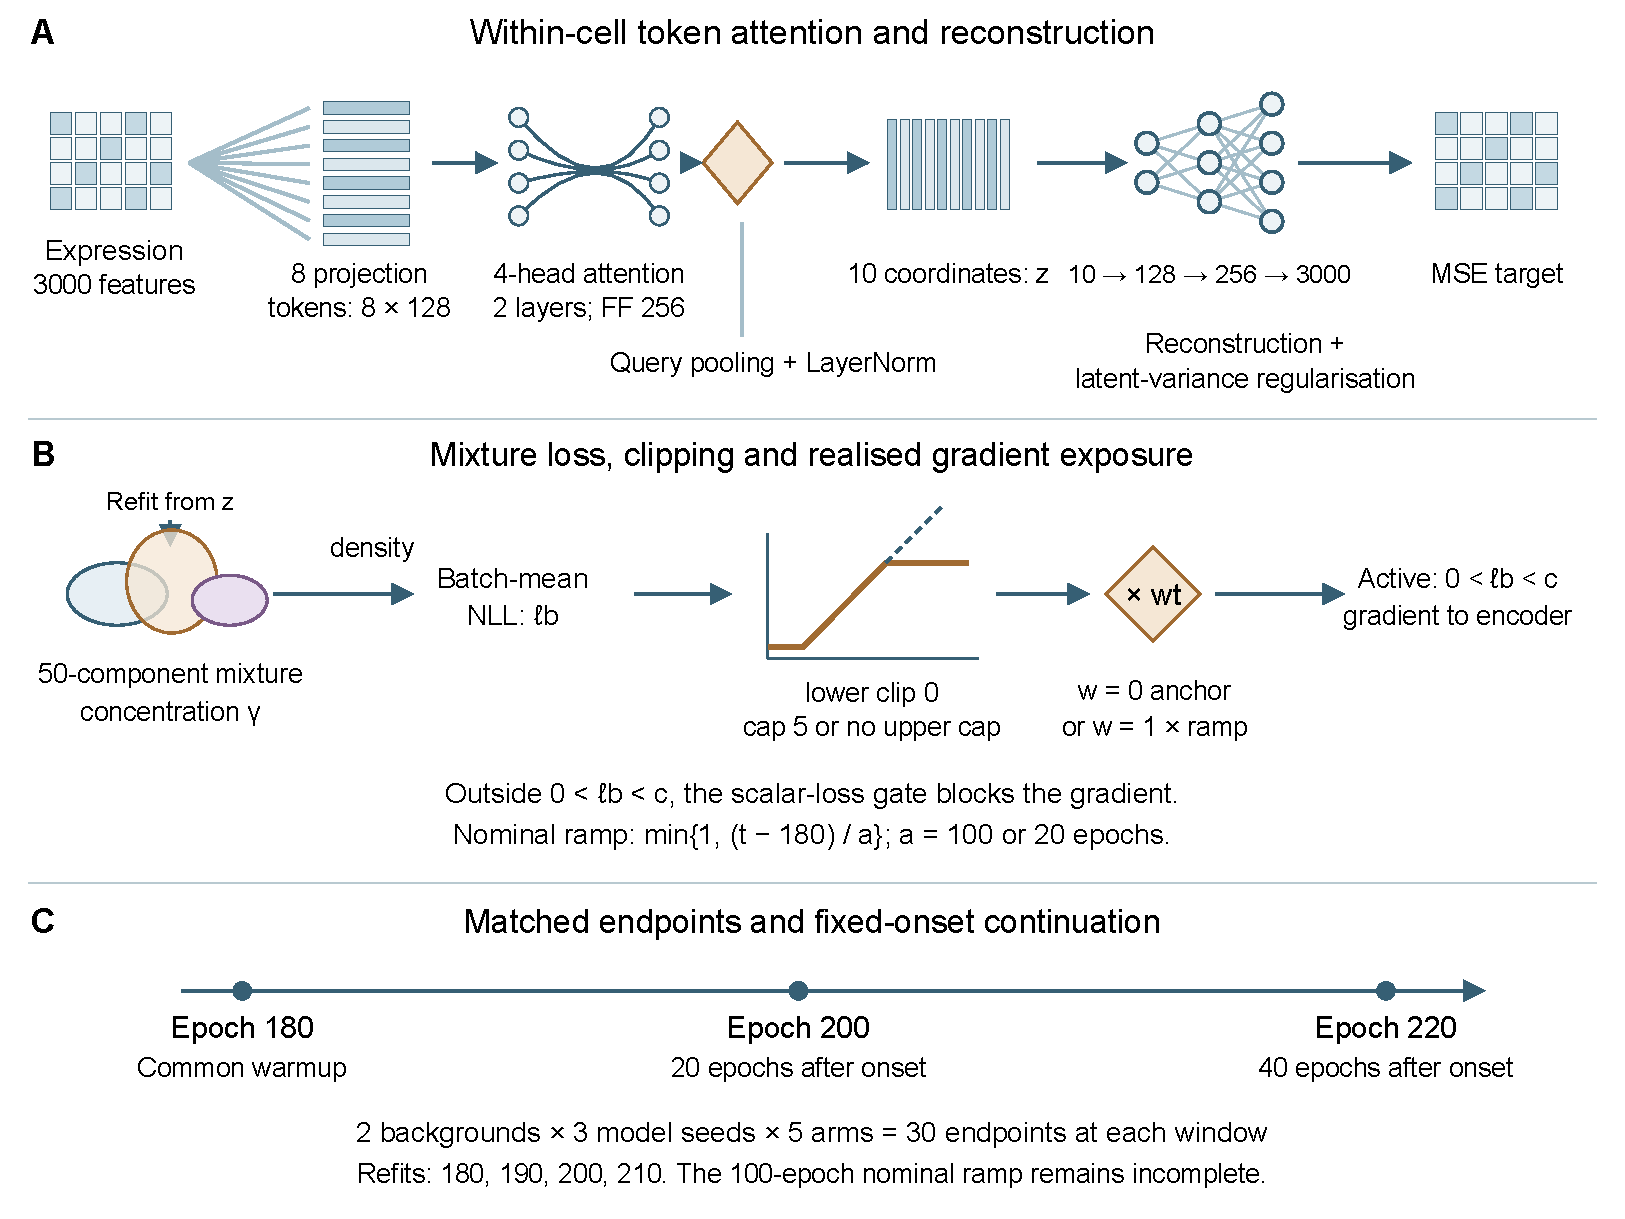
\includegraphics[width=\textwidth]{figures/architecture.pdf}
\caption{Attention representation and the controlled mixture-loss path.
A: eight 128-dimensional projection tokens pass through two four-head attention layers and learned-query pooling to ten deterministic latent coordinates. A $10\to128\to256\to3000$ decoder reconstructs normalized expression; the variance penalty remains active independently of mixture coupling. B: a 50-component diagonal density supplies a batch-mean NLL, clipped at zero and optionally five before weighting. The analytic transfer curve and Eq.~\ref{eq:active-gradient} identify the active gradient interval; its dashed extension removes the upper cap. C: six shared background--seed histories each produce four cap-by-ramp arms and an uncoupled anchor at epochs 200 and 220. Onset remains 180; $a=100$ is not a completed hundred-epoch intervention.}
\label{fig:arch}\end{figure}
\subsection{Encoder, decoder and fitted mixture}
The saved checkpoint tensors and the model source whose SHA-256 matches the factorial archive specify eight independent $3000\to128$ Linear--LayerNorm--GELU projections, learned token embeddings, two four-head attention layers with feedforward width 256, and one learned-query pooling operation. Attention acts on $[B,8,128]$ within cells; each head has width 32. Query pooling is related to Set Transformer~\cite{lee2019set}. Final LayerNorm~\cite{ba2016layer} and a $128\to10$ linear map give deterministic $z\in\mathbb R^{10}$. The decoder has widths $10\to128\to256\to3000$, with LayerNorm and GELU after its two hidden maps. Dropout is zero; the evaluated configuration has no variational sampling, bottleneck or batch-normalisation running statistics.

Mixture refits use diagonal-covariance \texttt{BayesianGaussianMixture} with 50 truncation components, concentration $\gamma=1$, mean-precision prior 0.1, $K$-means initialisation, at most 100 variational iterations and tolerance $10^{-3}$. Each fit adds Gaussian jitter of SD $10^{-6}$ using a recorded private seed offset by the refit epoch and fixes mixture random state 42. The exact seed rule belongs to the historical training drivers retained by the author; those drivers are not included in this release, and the supplied model snapshot alone does not reproduce that rule. Fitted parameters are held constant during encoder backpropagation between refits. Installed diagonal precision square roots are restricted to $[10^{-6},10]$; the terminal observer uses the estimator's unmodified fitted precisions. This numerical difference is retained when comparing the two estimators. Finite objective values do not imply variational convergence; saved convergence flags are audited separately.

\subsection{Objective and the historical confounding}
Let $X\in\mathbb R^{B\times G}$ denote the stored normalized expression supplied to both encoder and reconstruction target, $Z$ its ten-dimensional latent, and $s_j^2=(B-1)^{-1}\sum_i(z_{ij}-\bar z_j)^2$ its sample variance within the minibatch. The exact evaluated loss is
\begin{align}
 \mathcal L_b&=\frac{1}{BG}\sum_{i,g}(\hat x_{ig}-x_{ig})^2
       +\frac{10}{d}\sum_{j=1}^{d}\max(0,0.01-s_j^2)
       +w_t f_c(\ell_b),\label{eq:loss}\\
 \ell_b&=-\frac1B\sum_{i=1}^B\log\left[\sum_{k=1}^{50}
       \pi_k\mathcal N(z_i;\mu_k,\operatorname{diag}\sigma_k^2)\right],\qquad
 f_c(u)=\min\{c,\max(0,u)\}.\label{eq:gate}
\end{align}
Here $G=3000$, $B=128$, $d=10$, and $c=\infty$ means no upper cap. The variance penalty has coefficient 10 multiplying the mean shortfall over ten coordinates. Its threshold is in squared latent units; reconstruction is mean squared normalized-expression error. The density loss is in nats per cell in the fitted latent coordinate system. The implementation adds $10^{-10}$ inside logs of mixture weights and precision square roots. Despite the method name \texttt{\_dpmm\_loss\_kl}, the implemented term is a plug-in density NLL, not a variational assignment KL. There is no VAE KL term in this deterministic configuration.

Clipping acts on the batch-mean NLL, not separately on each cell's NLL. Away from boundary equalities, its contribution obeys
\begin{equation}
 \nabla_Z[w_t f_c(\ell_b)]
   =w_t\,\mathbf 1\{0<\ell_b<c\}\nabla_Z\ell_b.\label{eq:active-gradient}
\end{equation}
We check recorded nonzero gradients rather than infer them only from nominal weights; equality points follow the autodifferentiation implementation. This scalar-loss gate differs from global parameter-gradient norm clipping~\cite{pascanu2013difficulty}, applied after all loss terms are backpropagated. The schedule is
\begin{equation}
 w_t=w\min\{1,(t-180)/a\},\qquad t=180,\ldots,199,
\end{equation}
where $a$ is the nominal ramp horizon in epochs, not the observed intervention length. All arms end after the same 20 post-warmup epochs ($t=180,\ldots,199$); neither arm runs for 100 post-warmup epochs. At $\ell_b>c$, the upper
clamp's derivative is zero; this is a conditional statement, not a property
of every finite cap. The variational mixture implementation follows scikit-learn\cite{sklearn18bgm}. The installed precision is also capped by the model's
existing numerical rule, which is held fixed in the new experiment.

The historical capped configuration used $c=5,a=100$, whereas the uncapped
rerun used $c=\infty,a=20$. Across the 20-epoch coupling window, their nominal
summed weights are respectively $1.9w$ and $9.5w$ epoch-equivalents. Thus the
uncapped configuration changes both scalar-loss capping and fivefold nominal
exposure. Additional historical screens at caps 10 and 20 reproduced the
freeze at the tested schedule; they do not imply that every finite cap freezes.


\subsection{Data, evaluation and scope of replication}
The historical four-background panel comprises Setty haematopoiesis,
Dentate\cite{hochgerner2018conserved}, pancreatic endocrinogenesis (Endo)\cite{bastidas2019endocrinogenesis}, and Lung. The Lung file GSE130148 is adult human lung from
unaffected regions of surgical resections, not a lung-development cohort
\cite{vieirabraga2019lung}. Historical runs cap each background at 3,000
cells and 3,000 highly variable genes, use preprocessing and random cell-split
seed 42, and train seeds 0--2 with latent dimension 10 and mixture truncation
50. Normalisation and feature selection preceded the cell split. This is a
transductive representation experiment, not an independent-patient prediction
study. The historical training batch size is 128. A model seed is not a donor,
and biological state identity is not identified by these runs.
Model seeds quantify optimisation variability; cells, overlapping
splits and repeated scores are not independent biological replicates.

The original descriptive grid has four backgrounds, three seeds, four
coupling values $w\in\{0,0.5,1,2\}$ and two concentration values
$\gamma\in\{0.02,1\}$, with the other axis held at 1. Its 72 records include
12 duplicate operating-point specifications: $w=1$ and $\gamma=1$ specify the
same configuration. The 400-epoch Setty sensitivity has nine records, of
which the $\gamma=1$ records repeat the $w=1$ specification. These are not
additional independent replications. A 90\% warmup moves from epoch 180 to
360 when the total budget doubles; both intervention onset and duration
therefore change.

Edge survival is a reference-graph diagnostic against the same held-out
cells' PCA-50 representation. Both Euclidean 15-neighbour graphs exclude self and use union symmetrisation. For reference edge set $E_R$ and candidate shortest-path hop distance $h_C$, edge survival is $|E_R|^{-1}\sum_{(i,j)\in E_R}h_C(i,j)^{-1}$, with disconnected endpoints contributing zero. It is dimensionless and is not a cell-type or trajectory accuracy
measure. Reachability can remain one for a connected but rearranged graph.
Setty alone supplies Palantir branch probabilities for a five-fold $k$NN
regression probe, reported as $R^2$ at $k=15$\cite{setty2019palantir}.
These computed probabilities are an external computational annotation,
not prospective lineage tracing. A negative $R^2$ means worse prediction
than the fold-specific constant baseline; it does not establish biological
lineage destruction. A second historical branch score need not agree with
this local probe.

The latent $z\in\mathbb R^{10}$ is unconstrained. Applying softmax produces
ten coordinate weights, not fifty mixture responsibilities. The revised
RAAG-v2 scorer marks native-allocation scores as \texttt{non\_native} and
serializes their values as null. Softmax-coordinate coherence and perplexity
remain explicitly named coordinate diagnostics and do not support allocation
or cell-state claims. Gaussian conditional probabilities, where available,
are computed instead as
\begin{equation}
 r_{ik}=\frac{\pi_k\mathcal N(z_i;\mu_k,\Sigma_k)}
 {\sum_{j=1}^{50}\pi_j\mathcal N(z_i;\mu_j,\Sigma_j)}.
\label{eq:responsibility}
\end{equation}
These plug-in conditional probabilities are distinct from both the raw latent
and a full variational posterior over assignments.

UMAP panels use the 450 stored Setty test cells and the historical labels
0--9 produced by a $K$-means fallback. They are not curated cell-type labels.
The revised \texttt{umap-knn15-nonself-v2} purity uses each point's first 15
nonself neighbours. The former generator inadvertently omitted the first
nonself neighbour and included the sixteenth; the corrected-neighbour analysis rescores the unchanged
coordinates. Panel axes are independent UMAP coordinates without physical
units\cite{mcinnes2018umap}. Neither appearance nor label purity establishes
lineage recovery.

All new analyses are exploratory. The reporting and statistical interpretation were revised after inspecting the historical results; no prospective confirmatory significance is claimed. Per-seed values and paired contrasts remain visible.

\subsection{New matched factorial and measurement contract}
The checkpoint experiment declares two backgrounds (Setty, Endo), seeds 0--2, and four $w=1$
arms: cap 5 or no upper cap crossed with nominal ramp horizons $a=100$ or $a=20$. All arms are observed for the same 20 post-warmup epochs. A single $w=0$
anchor is sufficient because cap and annealing are structurally irrelevant
when the mixture coefficient is zero. There are six shared warmups and
thirty endpoint arms, not thirty independent initialisations.

Every background--seed pair starts from one autoencoder state. The entire
model, normalization parameters, AdamW state and NumPy/CPU/CUDA random
states are preserved at the absolute 180-epoch branch point. First-step and
warmup-boundary probes require identical model and optimiser hashes across
all five arms. Before mixture fitting, the arm-dependent loss path is inactive.
One private-RNG permutation is fixed per epoch and shared by all arms;
training and refit samples have the same order across arms. Setty has 2,100
training cells and 16 updates per epoch; Endo has 1,771 and 13. Batch size is
128 with the remainder dropped. Each arm completes 200 epochs with no early
stopping or validation selection, giving 3,200 or 2,600 total updates. AdamW
uses learning rate $10^{-3}$, decoupled weight decay~\cite{loshchilov2019decoupled} $10^{-5}$ and gradient clipping 10.

Refits occur at zero-indexed epochs 180 and 190 with deterministic private
jitter and a fixed mixture random seed. This deliberately matched schedule
is a new experiment, not bitwise replay of the historical shuffled-loader
procedure. Recorded endpoints include raw mixture loss, the fraction of
batches exceeding the cap, the mixture gradient norm with respect to $z$,
and the count of batches with both a nonzero gradient and a nonzero weight.
The last installed training mixture and a separate terminal full-training-set
observer are both saved with weights, means and precisions. We compute
Eq.~\ref{eq:responsibility}, Hungarian mean correspondences\cite{kuhn1955hungarian}, aligned
probability divergence and hard-assignment agreement; none defines a
biological state identity. Metric version is RAAG-v2, and all non-native
allocation values are null with explicit status.

\subsection{Fixed-onset checkpoint continuation and gradient dose}
Each of the thirty 200-epoch states is restored with its own model,
normalization parameters, optimizer tensors, installed mixture and
current mixture weight. Held-out latent arrays must replay bitwise before
any new update. Within each background--seed pair, continuation restores
the saved anchor random state for every arm and uses one shared deterministic
permutation for each epoch 200--219. The original absolute onset remains
180; the ramp is $w\min\{1,(t-180)/a\}$ throughout. The mixture refits at
zero-indexed epochs 200 and 210 on identical ordered subsets. No total-budget
warmup recalculation, early stopping or endpoint selection is used.
For every minibatch we save raw loss, cap activity, the unweighted clipped
mixture-loss latent-gradient norm $g_b$, nominal weight $w_b$, and their
product. The added-window gradient diagnostic is $\sum_b w_b g_b$; the
nominal epoch exposure is $\sum_b w_b$ divided by updates per epoch. A positive nominal
weight is not a dose: realised dose is recorded by the weighted gradient diagnostic.
Specifically, $g_b=\|\partial f_c(\ell_b)/\partial Z_b\|_F$ is the Frobenius norm over the entire $128\times10$ latent minibatch for the batch-mean loss, measured before global parameter-gradient clipping. It has loss-per-latent-unit scaling, is not a parameter-gradient norm and is not divided by the number of updates in the primary sum. A secondary per-update normalization checks the different Setty/Endo batch counts. We recompute every archived batch product, compare both endpoint arrays of each cap arm with its anchor, and calculate deletion of one background--seed warmup or one seed index across backgrounds. These exploratory influence checks use no inferential $p$ values.
Only epochs 200--219 have archived per-batch gradient dose. The 180--199 archive has active-batch aggregates but cannot support a full-window dose regression. We pair the added-window sum with anchor-adjusted edge change from epoch 200 to 220 within background--seed warmups. Twelve uncapped arm records share six warmups, and batches are not independent biological replicates. A hypothetical simultaneous rescaling of the ten-dimensional latent and Gaussian means by $s$ and covariances by $s^2$ shifts NLL by $10\log s$; applying this identity to archived raw losses is a gate-placement diagnostic, not a refitted or retrained endpoint.
The protocol adds $30\times20$ branch epochs, corresponding to 8,700
optimizer updates across the two background-specific batch counts.

\section{Results}
\subsection{Factorial evidence separates cap from nominal exposure}
All arms end after the same 20 post-warmup epochs; $a=100$ and $a=20$ specify nominal ramp horizons within that window. All six background--seed pairs pass initial-state, warmup-boundary,
minibatch, refit-subset and update-count gates. Both cap-5 arms bind on every
recorded coupling-window batch and have zero batches with an effective
mixture gradient. Their final latent arrays are byte-identical to the
uncoupled anchor in all six pairs. This establishes a cap-mediated freeze
for cap 5 in this experiment. It does not establish a freeze for an
arbitrarily large finite cap.

Removing the cap lowers edge survival at each fixed nominal ramp horizon in
all six pairs (Figure~\ref{fig:factorial}). Reducing the nominal horizon from $a=100$ to
$a=20$ within the same 20-epoch window leaves the capped latents unchanged but further lowers edge survival in
all six uncapped pairs. The historical uncapped difference therefore included
an exposure effect as well as cap removal. Table~\ref{tab:factorial} reports
all arms by background. Between 140 and 192 batches per uncapped $w=1$ arm
have both a nonzero mixture gradient and a nonzero weight, compared with
zero for capped arms and the anchor. Nominal ramp horizon alone does not
count effective interventions; the lower clip can also suppress the gradient.

The Setty branch probe separates the uncapped schedules. Its three values
are $0.653/0.718/0.684$ for the anchor and both capped arms,
$0.793/0.511/0.604$ for uncapped $a=100$, and
$-0.555/-0.266/0.347$ for uncapped $a=20$.
The slower uncapped schedule includes one improvement relative to the anchor;
a claim that removing the cap always lowers this branch score is unsupported.
All three faster-schedule values are lower than their paired slower-schedule
values. There is no Palantir endpoint for Endo.

The installed and terminal mixtures often disagree markedly in effective
occupancy (Table~\ref{tab:factorial}). For example, Setty uncapped $a=20$ has training occupancy $15.28/8.86/6.35$ but terminal observer occupancy
$11.72/49.80/49.81$. Both parameter sets and their conditional probabilities
are saved. They differ in refit time, sample size and installed precision
handling, so these are different estimators, not alternative counts of a
known biological state population.

An independent archive audit finds nonconvergence flags in 46 of the 60 recorded training refits (two per endpoint arm). Counts include repeated matched fits. This limits mixture-fit and occupancy interpretation, while the saved bound activity and exact capped-anchor equality remain directly checkable.

An initial production attempt stopped at the warmup-boundary equality gate
before any endpoint: loading an AdamW state without copying its tensors
mutated the reusable source state. The corrected driver deep-copies the
optimizer state before every fork. The failed attempt's 2,890 optimizer
updates are retained separately, as are 29 smoke updates and 60 successful
gate-probe updates. The completed experiment executes 24,360 unique scientific
updates by sharing warmup; the thirty endpoint histories together represent
87,000 updates. The failed attempt contributes no scientific endpoint.

\begin{figure}[htbp]\centering
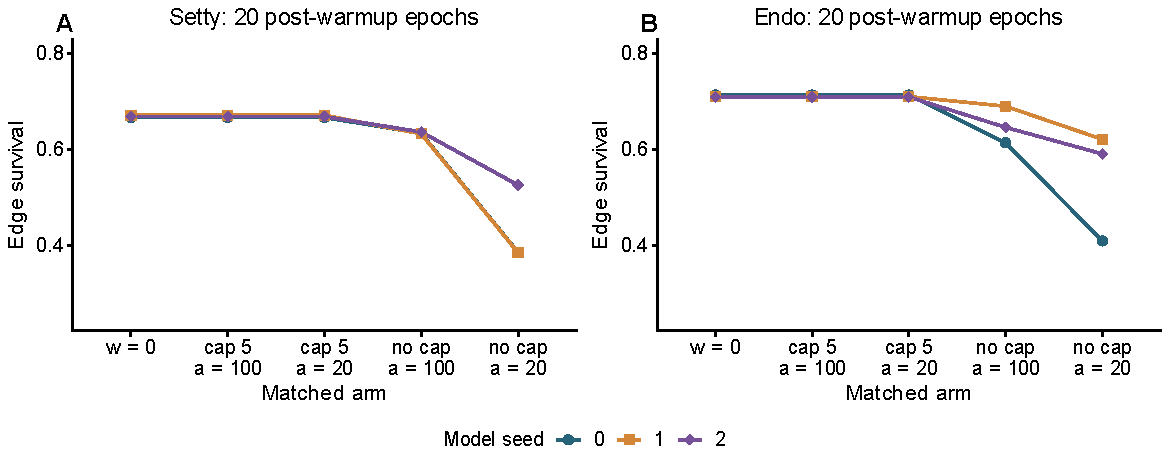
\includegraphics[width=\textwidth,height=0.70\textheight,keepaspectratio]{figures/factorial_edge.pdf}
\caption{All thirty matched factorial endpoints at epoch 200.
A: Setty; B: Endo. Edge survival compares each latent with PCA-50 neighbours of the same 450 or 380 held-out cells. Five categories cross cap 5/no cap with nominal horizon $a=100/20$ and include a $w=0$ anchor. Color/shape identify seeds in the shared key. Lines join matched categorical arms, not a continuous dose. Capped arms coincide with the anchor but retain separate records. Each arm receives twenty post-warmup epochs. There are six shared histories, with no seed averaging or error bars.}
\label{fig:factorial}\end{figure}

\begin{table}[htbp]\centering\small
\caption{Matched factorial summaries across three model seeds. Edge reports mean $\pm$ sample SD. $K_T$ and $K_O$ report seed means of last training-refit and terminal-observer effective occupancy, respectively. Gradient counts give the observed seed range of batches
with a nonzero mixture gradient and positive effective weight. They are not
independent biological observations.}
\label{tab:factorial}
\begin{tabular}{llrrrr}\toprule
Background & Arm & Edge, mean $\pm$ SD & $K_T$ & $K_O$ & Active batches\\\midrule
Setty & $w=0$ & $0.668\pm0.002$ & 9.27 & 9.48 & 0--0 \\
Setty & $c=5,a=100$ & $0.668\pm0.002$ & 9.27 & 9.48 & 0--0 \\
Setty & $c=5,a=20$ & $0.668\pm0.002$ & 9.27 & 9.48 & 0--0 \\
Setty & $c=\infty,a=100$ & $0.634\pm0.002$ & 24.04 & 48.83 & 179--184 \\
Setty & $c=\infty,a=20$ & $0.432\pm0.081$ & 10.16 & 37.11 & 175--192 \\
Endo & $w=0$ & $0.711\pm0.002$ & 8.86 & 8.68 & 0--0 \\
Endo & $c=5,a=100$ & $0.711\pm0.002$ & 8.86 & 8.68 & 0--0 \\
Endo & $c=5,a=20$ & $0.711\pm0.002$ & 8.86 & 8.68 & 0--0 \\
Endo & $c=\infty,a=100$ & $0.650\pm0.038$ & 31.02 & 48.16 & 148--155 \\
Endo & $c=\infty,a=20$ & $0.540\pm0.114$ & 23.86 & 35.49 & 140--157 \\
\bottomrule\end{tabular}\end{table}


\subsection{Historical branch and projection context}
The old capped grid has byte-identical latents across its coupling values
within each background--seed. The historical uncapped grid diverges. As shown
in Figure~\ref{fig:historical}, these are descriptive implementation records
with different annealing schedules; the factorial above supplies the matched
comparison. Its intervention does not retrospectively convert the historical
contrast into a one-factor experiment.

In the historical uncapped Setty grid, branch-probe $R^2$ is
$0.588/0.650/0.711$ at $w=0$, $0.116/0.547/-0.018$ at $w=1$, and
$0.001/-0.118/-0.315$ at $w=2$. At $w=2$, edge survival changes from
$0.665/0.671/0.665$ to $0.417/0.350/0.533$. This is evidence of a
representation cost under that recipe; it does not identify a general
attention or mixture failure. The concentration contrast also cannot be
called inert: on uncapped Endo, the historical coordinate diagnostic changes
by about $0.271$ and mean effective occupancy by about $23.0$; the Setty
occupancy change is about $12.8$. Effects are background- and endpoint-dependent.
\begin{figure}[htbp]
\centering
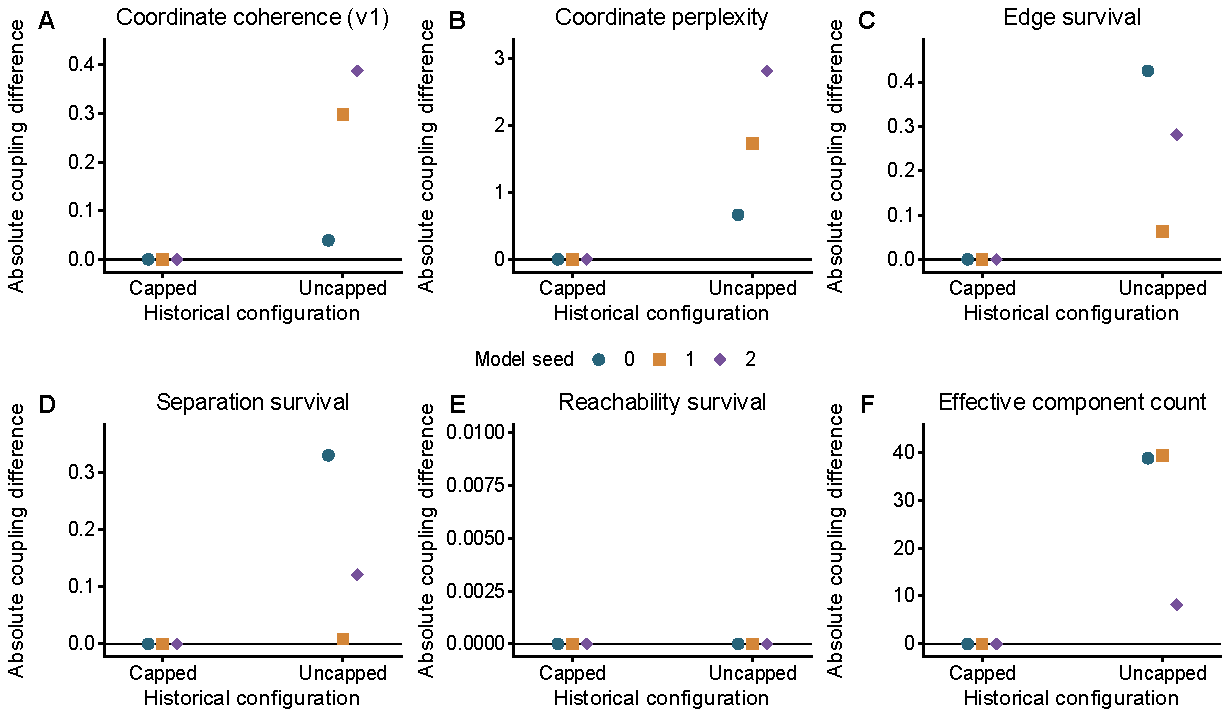
\includegraphics[width=0.96\textwidth,height=0.70\textheight,keepaspectratio]{figures/clamp_vs_unclamped.pdf}
\caption{Historical Setty absolute within-seed $w=1$ minus $w=0$ differences, $\gamma=1$, 200 epochs.
A--F: coordinate coherence (v1), coordinate perplexity, edge survival, separation, reachability and effective mixture occupancy. Each retains its own vertical scale. Historical capped ($c=5,a=100$) and uncapped ($c=\infty,a=20$) configurations differ in both cap and ramp. Color/shape and slight offsets distinguish three seeds; each panel retains six unaveraged points, with zero marked and no error bars. Coordinate diagnostics concern softmax of ten latent coordinates, not 50-component assignments. Occupancy concerns global mixture weights.}
\label{fig:historical}
\end{figure}

Figure~\ref{fig:umap} retains the original uncapped Setty coordinates.
The corrected first-15-nonself-neighbour purity is
$0.7591/0.7744/0.7770$ at $w=0$ and $0.2504/0.6618/0.3978$ at $w=1$
(Figure~\ref{fig:purity}). All three changes remain negative, but their
magnitudes differ considerably. The labels are the historical $K$-means
fallback, so the low-purity seed is not a demonstrated cell-type failure.
Historical $K_{>1\%}$ at uncapped $w=1$ is $43/50/1$; reporting those
three counts does not infer three biological state populations.
\begin{figure}[htbp]\centering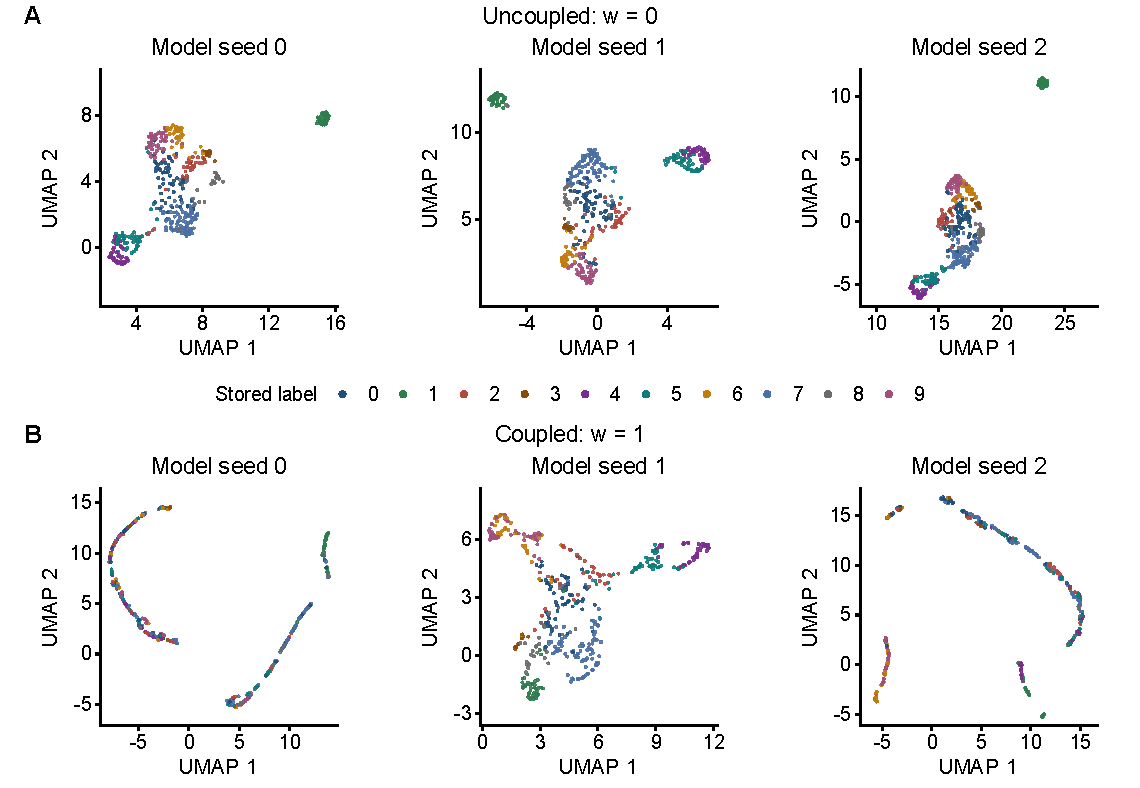
\includegraphics[width=0.96\textwidth,height=0.70\textheight,keepaspectratio]{figures/setty_umap.pdf}
\caption{Historical uncapped Setty UMAP at 200 epochs, $\gamma=1$.
Rows A/B: $w=0/1$; columns: seeds 0--2. Each tile retains 450 cells and unchanged coordinates, with no aggregation. The inter-row key maps historical $K$-means labels 0--9 to color; these are neither curated cell types nor mixture components. Coordinates are dimensionless, independently fitted and equal-aspect within tiles. Figure~\ref{fig:purity} rescores their first 15 nonself neighbours. Visual separation or clustering-label purity does not establish biological state discovery.}\label{fig:umap}\end{figure}
\begin{figure}[htbp]
\centering
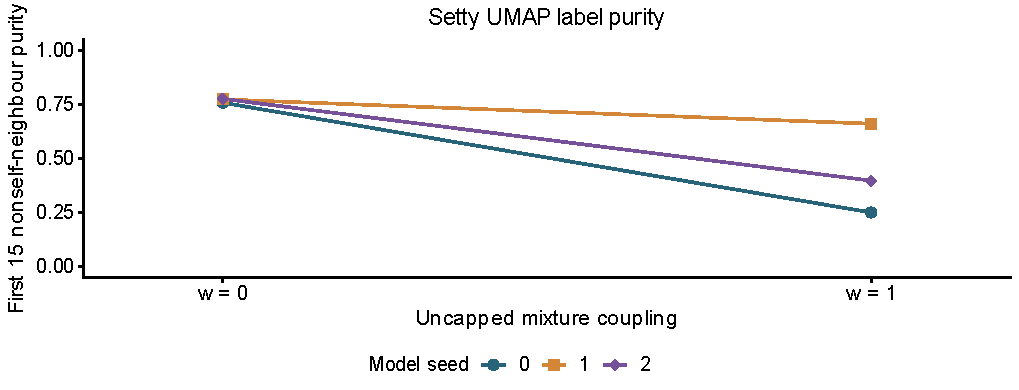
\includegraphics[width=0.96\textwidth,height=0.70\textheight,keepaspectratio]{figures/purity_callout.pdf}
\caption{Corrected historical Setty UMAP purity at $\gamma=1$, 200 epochs.
Each score averages, over 450 cells, the fraction of first-15 nonself neighbours sharing its $K$-means label. Color/shape identify seeds; lines join six $w=0/1$ projection summaries without seed averaging or error bars. Ranks 1--15 replace ranks 2--16 on unchanged coordinates; all paired differences remain negative. The unit is a model seed, and clustering labels do not provide lineage validation.}
\label{fig:purity}
\end{figure}


\subsection{A longer window separates nominal and realised exposure}
All thirty saved 200-epoch checkpoints pass bitwise latent replay before
continuation to epoch 220, adding 8,700 optimiser updates. The absolute
warmup remains 180, so this extends the observed coupling window from twenty
to forty epochs without completing the nominal hundred-epoch ramp.
During the added window, nominal weight sums are 5.9 epoch-equivalents for
$a=100$ and 20.0 for $a=20$, compared with 1.9 and 9.5 in the original
window. Despite those positive nominal sums, both cap-5 arms continue to
have zero effective mixture-gradient batches and remain byte-identical to
the anchor in all six pairs.

Uncapped arms have only 14--34 batches with positive weighted mixture
gradient during the added twenty epochs; lower clipping can make the other
batches inactive. Their summed weighted latent-gradient norms range from
17.14 to 46.60 for $a=100$ and from 100.20 to 161.09 for $a=20$.
Earlier uncapped arms had 140--192 active batches per 260 (Endo) or 320 (Setty), compared with 14--34 in the added window with the same respective denominators. The decrease in active batches is observable; a corresponding comparison of cumulative gradient sums is not.
This is a directly recorded gradient diagnostic, not a parameter-displacement
measure. At epoch 220, all six uncapped $a=20$ edge scores remain below
their paired $a=100$ scores (Figure~\ref{fig:extension}). Individual edge
scores can rise or fall relative to epoch 200, so more elapsed updates do
not imply a uniform trajectory of deterioration or recovery.

Across twelve uncapped arm records, Pearson correlation of added-window $\sum_b w_b g_b$ with anchor-adjusted edge change is 0.230 (Spearman 0.448), with Setty 0.773 and Endo 0.022 separately (six records per background). Dividing dose by each background's update count gives Pearson 0.213 and Spearman 0.371. In six within-warmup fast-minus-slow contrasts Pearson correlation is 0.628; removing one warmup gives 0.288--0.760, whereas removing seed index 0, 1 or 2 across both backgrounds gives 0.844, 0.802 or 0.040. The seed-2 omission is therefore particularly influential. These unstable exploratory correlations are not an independent dose--response curve or a causal effect of dose: gradient magnitude depends on the evolving representation and mixture. The $10\log s$ gate check places all uncapped $a=20$ batches below the zero floor for $s=0.5$, whereas $s=2$ places 98--184 above zero, compared with 20--34 at observed scale. Capped $a=20$ batches remain above the upper cap at all three tested hypothetical scales. These are same-log gate calculations, not predictions for rescaled training or refitted density.
\begin{figure}[htbp]\centering
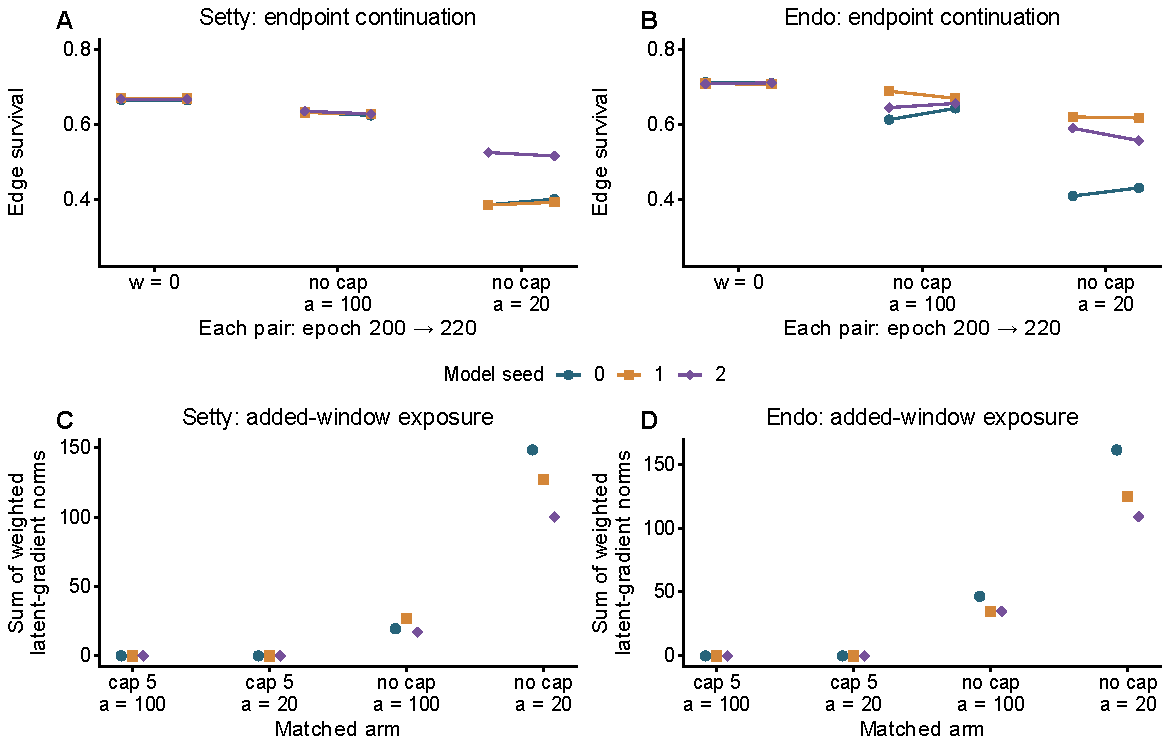
\includegraphics[width=\textwidth,height=0.70\textheight,keepaspectratio]{figures/window_extension.pdf}
\caption{Checkpoint continuation with onset fixed at epoch 180.
A/B: Setty/Endo edge survival; left/right points join epochs 200/220 within seed for the anchor and two uncapped horizons. Both capped arms coincide with the anchor. C/D: added-window $\sum_b w_b g_b$, with $g_b$ the Frobenius latent-gradient norm of the batch-mean clipped mixture loss. All four coupled arms, including zero-dose capped arms, are retained. Upper/lower panels contain 18/12 individual summaries, with a shared seed key and no seed averaging or error bars. Thirty restored arms share six histories, with 450 Setty/380 Endo test cells. Gradient sums are neither parameter displacement nor biological dose; the hundred-epoch ramp remains incomplete.}
\label{fig:extension}\end{figure}

\section{Discussion}
The factorial establishes that cap five suppresses the mixture gradient throughout the original measured window, while removing that cap changes the representation at each fixed nominal ramp horizon. Reducing the horizon changes the uncapped endpoints further but leaves the capped arms identical to their uncoupled anchors. This separates two interventions that had been changed together in the historical comparison. The result is a causal statement about the measured code path and operating points: a binding bound explains the frozen mixture contribution, and nominal ramp speed matters when that contribution is active. It is not evidence that every finite cap disables regularisation.

Direct gradient accounting is essential to that interpretation. The external coefficient, raw density loss and derivative of the transformed loss answer different questions. A positive coefficient does not imply a nonzero contribution, because the upper or lower bound may suppress the derivative. Conversely, an uncapped density term can be active for only part of the observed window. Counting batches with both positive weight and nonzero gradient therefore improves on simply reporting the configured coefficient. The continuation adds the sum of weighted latent-gradient norms as a descriptive exposure measure. That quantity records the implemented path, but is not a direct measure of parameter displacement or a biological treatment dose.
The early window lacks per-batch gradients; a cumulative 180--220 dose regression is not identifiable. A confirmatory analysis would require a frozen definition and scale of $g_b$, per-batch exposure in both windows, a prespecified endpoint and horizon, independent biological sampling units and a planned cluster-level analysis. Latent-scale and mixture-refit sensitivity require prospective controlled arms. Neither arm records nor minibatches create biological replication.

The extension observes forty post-warmup epochs while preserving absolute onset at 180. Full checkpoint restoration and a shared continuation stream retain the paired design. The hundred-epoch nominal ramp remains incomplete, and the extension does not establish long-run convergence.

A mechanism result does not imply that all downstream endpoints respond in the same direction. In the original factorial, the slower uncapped ramp improves the Setty branch probe for one seed relative to the anchor, although edge survival decreases in every paired uncapped comparison. The faster ramp yields lower branch scores than the slower ramp in all three seeds. These findings show why geometry and annotation prediction should be reported separately. A representation can reorganise its neighbourhoods while preserving or improving access to one computed signal. Selecting a single endpoint after seeing the results would obscure that heterogeneity and encourage a broader harm claim than the data support.

The mixture summaries add another distinction. Last-installed training parameters and a terminal observer can give substantially different effective occupancies, because they differ in time, fitting sample and precision handling. Saving complete parameter sets permits their conditional probabilities to be reconstructed and compared. It does not identify one set as the true biological partition. Even under idealized sampling, mixture-component counts need not consistently estimate a population's number of groups~\cite{miller2014inconsistency}; our entropy-based occupancy is a further descriptive quantity. Hungarian matching of means provides a geometric correspondence, not persistent component identity. Component labels are exchangeable, and the encoder changes their coordinate system. Assignment divergence remains a model diagnostic rather than evidence of population birth or death.

The convergence audit adds a concrete numerical limitation: 46 of 60 recorded training refit operations at epochs 180 and 190 did not meet the estimator's tolerance within 100 iterations. Matched arms repeat some identical refits, so this denominator counts recorded operations rather than independent trials. Continuation and terminal-observer convergence flags were not archived. Finite fitted objectives and the directly observed cap gate still establish the measured gradient behavior, but cannot validate a converged mixture solution. Occupancy and uncapped endpoint sensitivity to refit tolerance, iteration budget and precision handling remain untested.

Thirty endpoint arms arise from six shared background--seed histories, not thirty independent initialisations. Batch logs increase measurement resolution without adding datasets. Gate probes and the failed warmup-boundary attempt remain in computational accounting, but contribute no scientific endpoints or additional replication.

Generalisation remains limited by the experimental scope. Only two backgrounds and three optimisation seeds enter the controlled factorial, with transductive preprocessing and a fixed latent dimension, truncation, optimiser and numerical precision rule. Historical four-background sweeps add descriptive context but do not broaden the randomised comparison beyond those controls. The Palantir probe is available only for haematopoiesis, and historical projection labels are clustering assignments rather than curated cell types. Sample-level validation and preprocessing fitted exclusively to training samples would address different deployment questions. The present continuation also tests one additional window length; it does not establish asymptotic convergence of either the encoder or the mixture estimator.

Reports of regularisation should retain raw objectives, bound activity, schedules, elapsed windows, nonzero-gradient batches and checkpoint state. Here those records distinguish an erased mixture contribution from the seed-dependent representation changes under uncapped schedules. Attribution remains conditional on the measured implementation and operating points.

\FloatBarrier
\section{Declarations}
\noindent\textbf{Data and code availability}\par\nobreak
The study-specific source repository is \url{https://github.com/PeterPonyu/mixture-regularisation-gating}; the versioned research archive is \url{https://doi.org/10.5281/zenodo.22914503}. The archive contains the manuscript, vector figures, thirty continuation endpoints, six schedules, saved per-batch exposure records, mixture parameters and analysis code. CPU commands reproduce exposure accounting and robustness checks. Model checkpoints are supplied separately within this archive. The retained model source is an inspection snapshot, not a complete training library; raw-data preprocessing and historical graph rescoring are outside the verified scope. The repository README gives the dependency requirements, commands and checksums. Source studies and their data-access conditions are identified in Materials and Methods and the bibliography. Author-owned software is MIT licensed; the author's manuscript, figures, generated results and weights are CC BY 4.0. Third-party data and annotations retain their original terms.

\noindent\textbf{Ethics approval and consent}\par\nobreak
The reported work is a computational reanalysis of existing single-cell datasets; no new participant recruitment or animal experiment is described. Study-specific ethics review or exemption information, consent-to-participate information, and consent-for-publication declarations have not been established in this report. No ethics approval, exemption or consent status is inferred from dataset availability.

\noindent\textbf{Funding}\par\nobreak
This research received no funding.

\noindent\textbf{Author contributions}\par\nobreak
Zeyu Fu is the sole author of this manuscript. The affiliation and contact address are printed on the title page. The author is responsible for the manuscript and its computational analyses.

\noindent\textbf{Competing interests}\par\nobreak
The author declares no competing interests.

\noindent\textbf{Acknowledgements}\par\nobreak
The author acknowledges the researchers who made the cited source datasets and software available.

{\bibliographystyle{plainnat}\bibliography{standalone-assets/refs,extra}}
\end{document}
